\subsection{Physics capabilities}
\label{sec:physics_capabilities}

``The code needs to be able to give reliable predictions of:
\begin{itemize}
\item[$\bullet$] Divertor loads:
\begin{itemize}
\item[$\bullet$] Reliable calculation of upstream particle and heat flux
	profiles: proper drift physics and upstream turbulence;
\item[$\bullet$] Divertor turbulence: turbulence spreading in the divertor
	region, effect of magnetic shear next to the X-point(s) to understand
	upstream/downstream connection;
\item[$\bullet$] Multifluid capacity to model radiation and detachment physics;
\item[$\bullet$] Reliable calculation of the electric field (collisionless
	physics near the separatrix, proper reflection of neutrals at the
	target);
\item[$\bullet$] Able to capture in/out and top/down asymmetries (geometry,
	drifts, radiation and detachment)
\end{itemize}
\item[$\bullet$] Wall loads:
\begin{itemize}
\item[$\bullet$] Should be able to predict filamentary transport and role of
	hot ion confinement (wall erosion)
\item[$\bullet$] Should calculate radiation and neutral loads (may require
	dedicated modules, same for divertor loads);
\end{itemize}
\item[$\bullet$] Impurity transport, pumping and fueling:
\begin{itemize}
\item[$\bullet$] Ability to track low (He Be), medium (C, N, Ne) and high Z
	impurities (W, Ar, Xe) with multiple charge states;
\item[$\bullet$] Reliable kinetic modelling of neutrals to assess fueling and
	pumping capacity;
\item[$\bullet$] Ability to handle non-trace species (D, T, He, seeded
	species), which requires new closures for the equations (if fluid,
	beyond Braginskii $\implies$ Zhdanov or better);
\item[$\bullet$] Accurate model of friction forces (turbulence + neoclassical
	on open field lines);
\item[$\bullet$] In high fidelity models, the code should be able to simulate
	localized gas puffs, via injection of neutral particles.
\item[$\bullet$] Dust  the code should enable coupling to codes to simulate
	dust generation, transport and ablation, via exchange of fluxes and
	sources.''
\end{itemize}
\end{itemize}



\paragraph{Physics models.}
Many points in this section relate to the physics model.
As we have alluded to above, the actual physics model used is the
responsibility of the user;
so, for example, it will necessary for users to derive an accurate model for
turbulent friction.
Moreover, as \nep\ will initially be an edge code, only electromagnetic
radiation from the edge plasma will be calculated, and an additional model will
be required for radiation for the core plasma. 
%{\blue Is that what is meant about radiation?}
Nonetheless, we plan to facilitate models which have the listed properties.
In particular, our meshing approach will allow accurate representation of the
walls and divertor.
Thus powerful and flexible source/sink models may be used, for both volumes and
surfaces.

\nep\ code will also be capable of representing scales on which filamentary
transport has been calculated to occur.
The code will only produce fluxes however, and it will be up to the user to
calculate wall erosion.



\paragraph{Validation, Verification and Uncertainty Quantification (VVUQ).}
Naturally, when the solution of a problem is unknown, it is difficult to assess
whether the provided answer is reliable as requested in the first line of the current section.
Therefore we are integrating \nep\ with a suite of tools for VVUQ to enable
validation of code outputs against experimental results, and provide a error
bars for code outputs due to the uncertainty in the code inputs.
As allowed by error estimates, models of different complexity will be used
to predict key properties of the SOL, see \Fig{dimensions2}.
\begin{figure}
\centerline{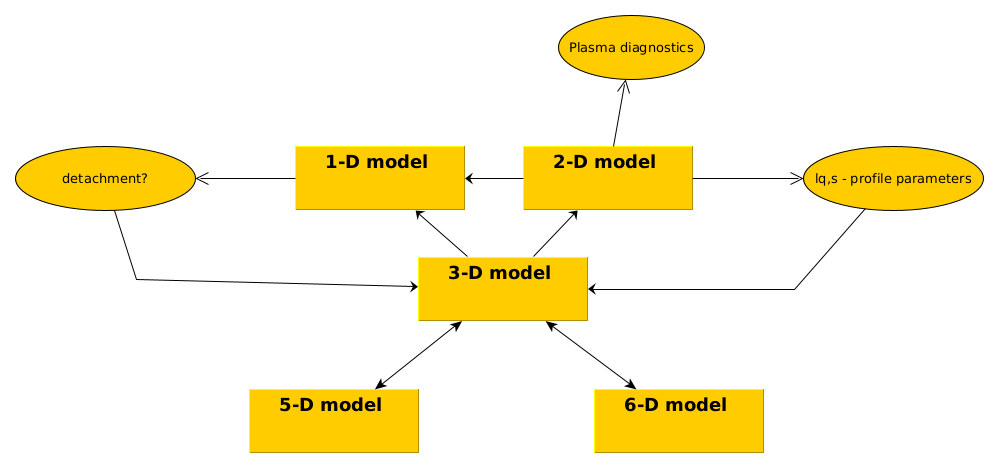
\includegraphics[width=0.7\textwidth]{./pics/dimensions2.png}}
\caption{
Project software will integrate a range of models of different complexity, here
indicated by their dimensionality.
\label{fig:dimensions2}}
\end{figure}
